\begin{figure}[th]
    \vspace{-0.5cm}
    \centering
    % 裁剪图片边缘可能存在的白色区域（根据实际情况调整参数）
        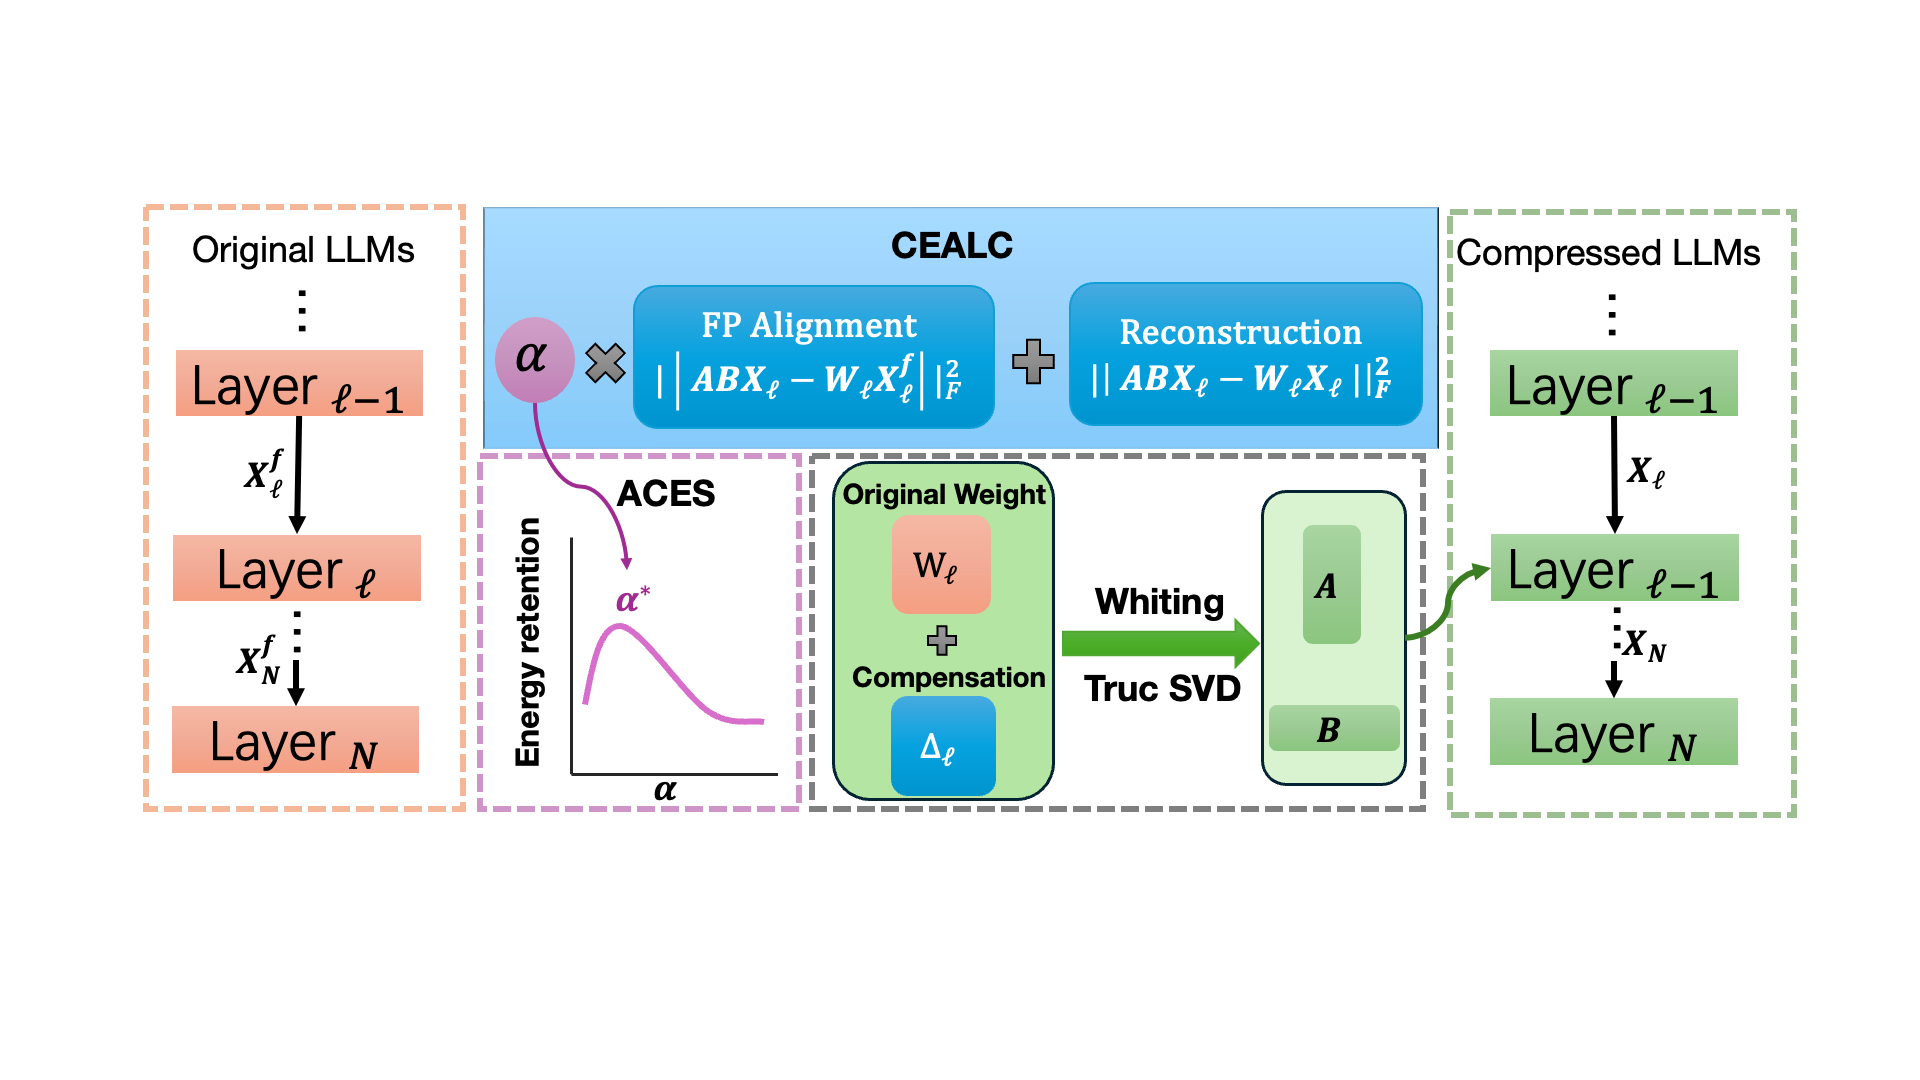
\includegraphics[width=1\linewidth, trim=55 60 55 60, clip]{figs/main.png}
    % 调整标题与图片的距离
    \vspace{-1.5cm}
    \caption{Overview of the proposed SAES-SVD framework.}
    \label{fig:main}  % 标签使用冒号分隔符，符合LaTeX规范
    % 调整图与下文的距离
    \vspace{-0.2cm}
    \end{figure}